
%# Miguel Angel Luque Fernandez, Daniel Redondo Sanchez and Michael Schomaker
%# American Journal of Public Health (AJPH)
%# Letter to the Editor 
%# Title:
%# Evaluating the effectiveness of public health interventions under non-collapsibility 
%# of the marginal odds ratio and effect modification: A Monte Carlo Simulation comparing classical
%# multivariable regression adjustment versus the G-Formula based on a cancer epidemiology illustration
%
%# Copyright (c) 2018  <Miguel Angel Luque-Fernandez, Daniel Redondo Sanchez and Michael Schomaker>
%# Permission is hereby granted, free of charge, to any person obtaining a copy
%# of this software and associated documentation files (the "Software"), to deal
%# in the Software without restriction, including without limitation the rights
%# to use, copy, modify, merge, publish, distribute, sublicense, and/or sell
%# copies of the Software, and to permit persons to whom the Software is
%# furnished to do so, subject to the following conditions:
%# The above copyright notice and this permission notice shall be included in
%# all copies or substantial portions of the Software.
%# THE SOFTWARE IS PROVIDED "AS IS", WITHOUT WARRANTY OF ANY KIND, EXPRESS OR
%# IMPLIED, INCLUDING BUT NOT LIMITED TO THE WARRANTIES OF MERCHANTABILITY,
%# FITNESS FOR A PARTICULAR PURPOSE AND NON-INFRINGEMENT. IN NO EVENT SHALL THE
%# AUTHORS OR COPYRIGHT HOLDERS BE LIABLE FOR ANY CLAIM, DAMAGES OR OTHER
%# LIABILITY, WHETHER IN AN ACTION OF CONTRACT, TORT OR OTHERWISE, ARISING FROM,
%# OUT OF OR IN CONNECTION WITH THE SOFTWARE OR THE USE OR OTHER DEALINGS IN
%# THE SOFTWARE.

\documentclass{article}\usepackage[]{graphicx}\usepackage[]{color}
%% maxwidth is the original width if it is less than linewidth
%% otherwise use linewidth (to make sure the graphics do not exceed the margin)
\makeatletter
\def\maxwidth{ %
  \ifdim\Gin@nat@width>\linewidth
    \linewidth
  \else
    \Gin@nat@width
  \fi
}
\makeatother

\definecolor{fgcolor}{rgb}{0.345, 0.345, 0.345}
\newcommand{\hlnum}[1]{\textcolor[rgb]{0.686,0.059,0.569}{#1}}%
\newcommand{\hlstr}[1]{\textcolor[rgb]{0.192,0.494,0.8}{#1}}%
\newcommand{\hlcom}[1]{\textcolor[rgb]{0.678,0.584,0.686}{\textit{#1}}}%
\newcommand{\hlopt}[1]{\textcolor[rgb]{0,0,0}{#1}}%
\newcommand{\hlstd}[1]{\textcolor[rgb]{0.345,0.345,0.345}{#1}}%
\newcommand{\hlkwa}[1]{\textcolor[rgb]{0.161,0.373,0.58}{\textbf{#1}}}%
\newcommand{\hlkwb}[1]{\textcolor[rgb]{0.69,0.353,0.396}{#1}}%
\newcommand{\hlkwc}[1]{\textcolor[rgb]{0.333,0.667,0.333}{#1}}%
\newcommand{\hlkwd}[1]{\textcolor[rgb]{0.737,0.353,0.396}{\textbf{#1}}}%
\let\hlipl\hlkwb

\usepackage{framed}
\makeatletter
\newenvironment{kframe}{%
 \def\at@end@of@kframe{}%
 \ifinner\ifhmode%
  \def\at@end@of@kframe{\end{minipage}}%
  \begin{minipage}{\columnwidth}%
 \fi\fi%
 \def\FrameCommand##1{\hskip\@totalleftmargin \hskip-\fboxsep
 \colorbox{shadecolor}{##1}\hskip-\fboxsep
     % There is no \\@totalrightmargin, so:
     \hskip-\linewidth \hskip-\@totalleftmargin \hskip\columnwidth}%
 \MakeFramed {\advance\hsize-\width
   \@totalleftmargin\z@ \linewidth\hsize
   \@setminipage}}%
 {\par\unskip\endMakeFramed%
 \at@end@of@kframe}
\makeatother

\definecolor{shadecolor}{rgb}{.97, .97, .97}
\definecolor{messagecolor}{rgb}{0, 0, 0}
\definecolor{warningcolor}{rgb}{1, 0, 1}
\definecolor{errorcolor}{rgb}{1, 0, 0}
\newenvironment{knitrout}{}{} % an empty environment to be redefined in TeX

\usepackage{alltt}
\usepackage[landscape]{geometry}
\usepackage{pgf,tikz}
\usetikzlibrary{positioning}
\IfFileExists{upquote.sty}{\usepackage{upquote}}{}

\begin{document}
\begin{center}
\begin{landscape}
\scalebox{1.4}
{
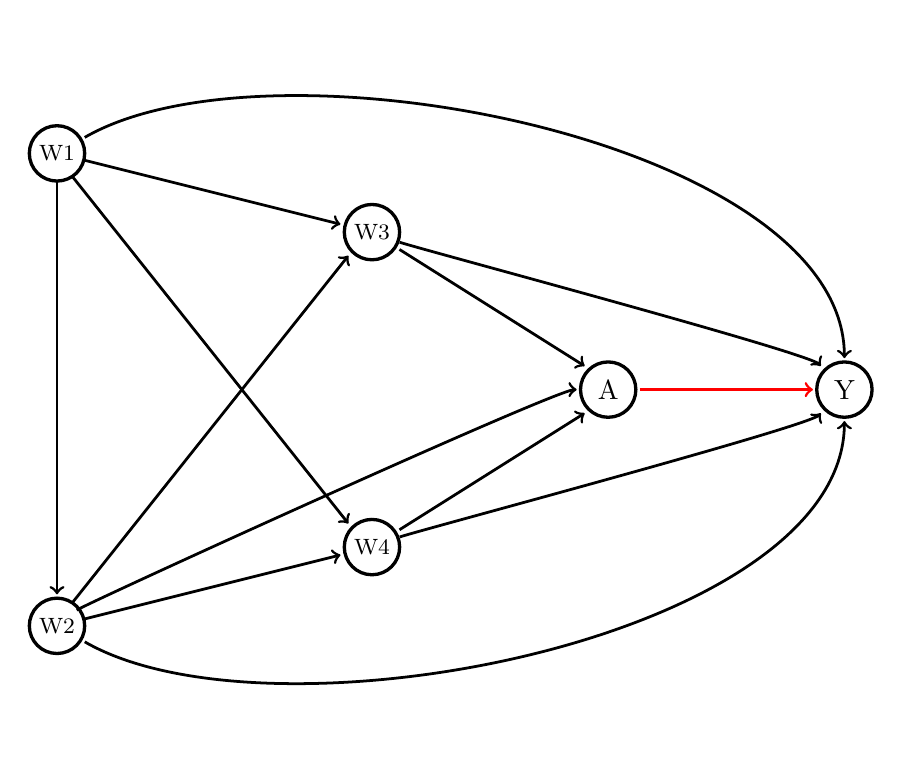
\begin{tikzpicture}
\draw[very thick] (-5,0) circle (10pt); %W2
\draw[very thick] (-5,6) circle (10pt); %W1
\draw[very thick] (-1,5) circle (10pt); %W3
\draw[very thick] (-1,1) circle (10pt); %W4
\draw[very thick] (2,3) circle (10pt); %A
\draw[very thick] (5,3) circle (10pt); %Y
  \draw (-5,0) node[font=\footnotesize] (w1) {W2};
  \draw (-5,6) node[font=\footnotesize] (w2) {W1};
  \draw (-1,5) node[font=\footnotesize] (w3) {W3};
  \draw (-1,1) node[font=\footnotesize] (w4) {W4};
  \draw (2,3) node (a) {A}; \draw (5,3) node (y) {Y}; %
  %----w1----%
  \draw[line width=1,->] (-4.8,0.3) -- (-1.3,4.7);
  \draw[line width=1,->] (-5,5.65) -- (-5,0.4);
  \draw[line width=1,->] (w1) -- (-1.4,0.9);
  \draw[line width=1,->] (-4.75,0.2) to [out=30,in=180, looseness=0.1] (1.6,3);
  \draw[->, line width=1] (w1) to [out=-30,in=-90, looseness=0.7] node[above,font=\footnotesize]{} (5,2.6);
  %----w2----%
  \draw[black,line width=1,->] (w2) -- (-1.4,5.1);
  \draw[black,line width=1,->] (-4.8,5.7) -- (-1.3,1.3);
  \draw[->, line width=1] (w2) to [out=30,in=90, looseness=0.7] node[above,font=\footnotesize]{} (5,3.4);
  %----w3----%
  \draw[black,line width=1,->] (w3) -- (1.7,3.3);
  \draw[black,line width=1,->] (w3) to [out=-20,in=130, looseness=0.1] (4.7,3.3);
  %----w4----%
  \draw[black,line width=1,->] (w4) -- (1.7,2.7);
  \draw[black,line width=1,->] (w4) to [out=20,in=-130, looseness=0.1] (4.7,2.7);
  %----w2----%
  \draw[red,line width=1,->] (2.4,3) -- (4.6,3);
\end{tikzpicture}
}
\end{center}
\end{document}
